%%%%%%%%%%%%%%%%%%% Figure 2 Bathymetry and currents in the Drøbak area %%%%%%%%%%%%%%%
\begin{figure}[t]
 \begin{center}
  \begin{pspicture}(0,0)(15,8.5)
% Include graphs
   \rput[tl](-0.1,9.5){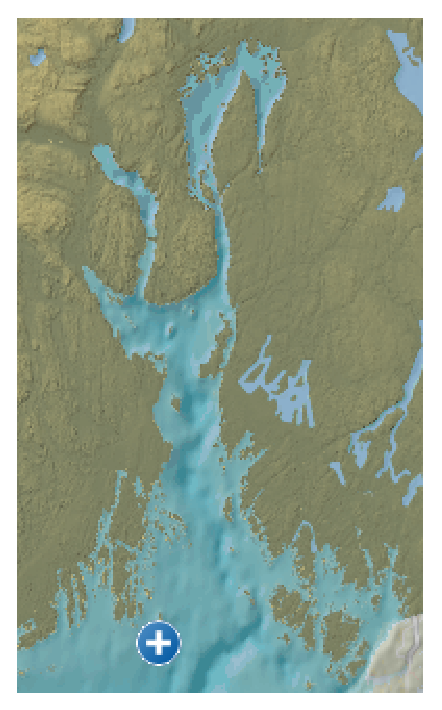
\includegraphics[height=8.5cm]{dyp}}
   \rput[tr](  15,9.5){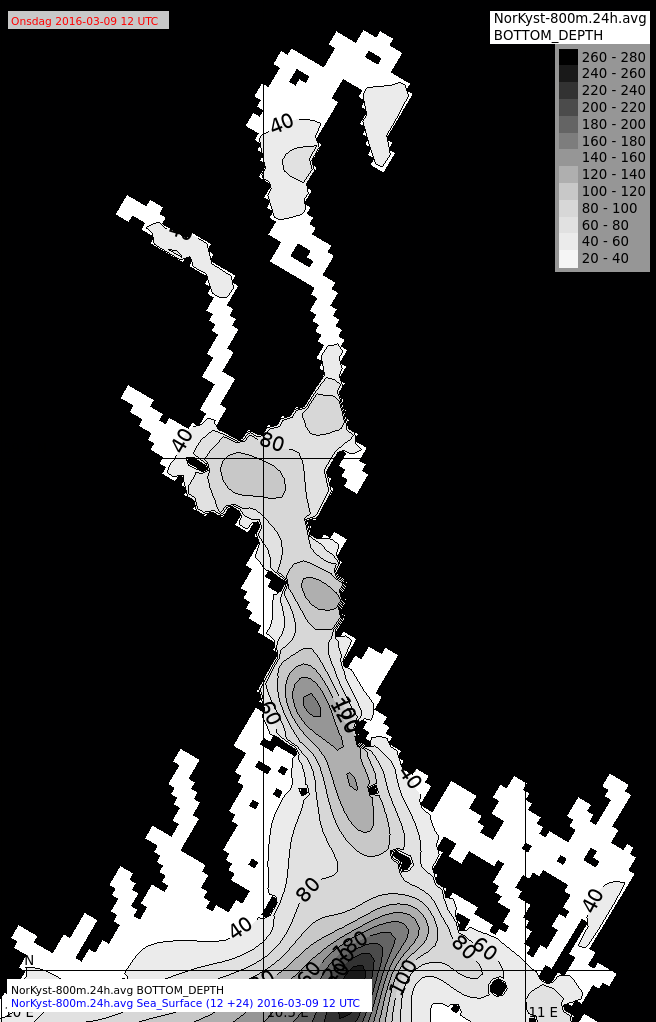
\includegraphics[height=8.0cm]{NorKyst800_topo_oslofjord}}
  \end{pspicture}
  \caption{\small The irregular coastline geometry and topography in the Oslofjord as portrayed in the FjordOs CL model (left) and the NorKyst800 model (right). The color bar (grayscale) indicate depth in meters.}
  \label{fig:hvaler2}
 \end{center}
\end{figure}

